\documentclass[11pt,letterpaper]{article}

\usepackage{amsfonts}
\usepackage{amsmath}
\usepackage{amssymb}
\usepackage[title]{appendix}
\usepackage{color}
\usepackage{csquotes}
\usepackage[margin=1in]{geometry}
\usepackage{graphicx}
\usepackage{listings}
\usepackage{multirow}
\usepackage{pifont}
\usepackage{tabularx}
    \newcolumntype{L}{>{\raggedright\arraybackslash}X}
\usepackage[usenames,dvipsnames,table]{xcolor}
\usepackage{xspace}
\usepackage{url}

\definecolor{cream}{RGB}{254,249,231}
\lstset{
    backgroundcolor=\color{cream},
    breaklines=true,
    basicstyle=\ttfamily\footnotesize,
    keepspaces=2,
    escapeinside={(*@}{@*)},
}

\newcommand{\parhead}[1]{\medskip \noindent \textbf{#1}~~}
\newenvironment{widelist}{\begin{list}{$\bullet$}{\setlength{\leftmargin}{.40cm}\setlength{\itemsep}{.00cm} }}{\end{list}}
\newcommand{\cmark}{\ding{108}}
\newcommand{\xmark}{ }
\newcommand{\pmark}{\ding{109}}
\newcommand{\name}{Phoenix\xspace}
\newcommand{\Name}{Phoenix\xspace}

\title{PhD Proposal}
\author{Stephen Herwig}
%\date{July 2, 2019}
\begin{document}
\maketitle
\begin{abstract}

Organizations shift the deployment of their services to untrusted third
parties, such as cloud infrastructures, content delivery networks, or email
providers, in order to reduce costs, increase availability, or gain
additional protections inherent to these hosting environments.
%
Unfortunately, such a shift poses a security tradeoff: third-parties that
provide or host the application potentially gain access to sensitive
information about the organization or its clients.


In my proposal, I ask whether it is possible to run legacy application binaries
with confidentiality and integrity guarantees that reflect the
organization's trust with respect to the application and its deployment
setting.
%
The constraint of running unmodified, legacy applications implies that the
enforcement of such guarantees is the responsibilty of the applications's
run-time execution environment. 
%
Since the execution environment is transparent to the application, the insight
is that it may be modified, partitioned, and distributed across domains of
varying trustworthiness, so as to reflect the security goals.


In the first part of my proposal, I review my prior work in extending a
library operating system that runs within an Intel SGX secure hardware
enclave, so as to support running a broader set of trusted, legacy,
applications in untrusted environments.
%
In the second part, I propose a new run-time system, \emph{Gemini}, that is
agnostic to the availability of secure hardware and the trustworthiness of
the application.
%
Gemini presents two complementary abstractions: \emph{distributed containers},
where organizations pin sensitive data to domains that they trust, and
\emph{policy monitors}---modules that an organization installs in a trusted
environment to enforce expected behavior of untrusted applications.
%
I present the design of Gemini and propose a set of evaluations for assessing
its correctness and performance.

\end{abstract}

\section{Introduction}
\label{sec:intro}
%    What problems are you trying to solve
%    carve out the space
%
%   We need cover concepts/problems that are common to all
%   the deployment stragegies, as well as define common terms here.

We define availability as the ability for a service to respond to
client requests at a desired quality of service (such as request latency),
as well as scale to a given throughput.
%
Thus, availability is an umbrella over the related concerns of
service scaling (as by service replication), load-balancing, and defense
against denial-of-service attacks.
%

\section{Problem and Goals}
\label{sec:background}

\subsection{Applications}

I focus on two use cases that involve multiple parties cooperatively running
an application where the input of at least one party is confidential:
(1) outsourcing TLS-based applications to a third-party, and (2)
analyzing the private data of multiple parties.


\parhead{Outsourcing TLS applications}
%% setup
I consider a company using a third-party, such as a cloud host or cloud
service, to operate an application server.
%
A common case is a company using a content delivery network (CDN) to
host their web content, and optionally manage their DNS and mail servers.
%
Virtually all of the most popular websites (and a very long tail
of unpopular websites) use one or more CDNs to help reliably host
their content~\cite{key-sharing}. 
%
Historically, CDNs have been thought of as a massive web
cache~\cite{cdn-on-demand}, but today’s CDNs play a critical role in achieving
the performance and security that the web relies on~\cite{securing-cdns}.

%% why a problem? status quo?
As a CDN requires the company's private TLS key to serve content over HTTPS,
the \emph{status quo} is for the company to share or otherwise entrust the CDN
with the application's private keys.
%
Indeed, CDNs have amassed the vast majority of private keys on the
web~\cite{key-sharing,when-https-meets-cdn}.
%
This has significant implications on the trust model of the PKI and the web
writ large, as the CDNs  can arbitrarily impersonate any of their customers.


\parhead{Collaborative Data Processing}
%% setup
I consider a multi-party setting, where the parties agree on an analysis to be
performed, and where the aggregate input for the analysis consists of the
confidential, local, data sets of each party.
% 
The parties themselves might be mutually distrustful, or may simply be
prevented by law from sharing their data.
%
The purpose of the analysis is to process the data sets to determine some
non-confidential result.
%
% TODO: cite
Common cases include a consortium of hospitals that want to pool their medical
records for research, but cannot lawfully disclose arbitrary patient records,
or a financial services industry  that must engage in a regulatory stress test,
but where each member bank is unwilling to disclose account details
with other financial institutions.


In such situations, the members must either agree on a trusted intermediary to
aggregate and analyze the data, or the analysis must be compartmentalized to
each specific party, rather than performed system-wide  over all parties
together.


%With federated databases, the result may be the cardinality of an intersection
%across the datasets.
%
%With federated learning, the result may be the global model parameters (such
%as the weights of a deep neural network), derived from the aggregation of the
%parameters from each party's locally-trained model.


\subsection{Goals}
At a high-level, my goal is to make heterogeneous trust a concern
of the application's run-time execution environment, rather than a concern of
the application developer.
%
I distill my overarching goal down to three specifics:

\begin{enumerate}
\item \textbf{Preserve confidentiality of private data:}
    The execution environment \emph{must} maintain the confidentiality of the
    private keys and private data sets of each party.

\item \textbf{Ensure data integrity:} 
    The execution environment \emph{should} preserve the integrity of each
    party's data.

\item \textbf{Require minimal changes to existing applications:}
    The execution environment \emph{should} maintain the abstraction of a
    monolithic application; if the run-time partitions the application
    across trust domains or otherwise uses a distributed execution
    environment, such an environment \emph{should} be transparent to the
    application.  
    %
    This requirement also implies that trust \emph{should} be
    expressible as a policy configuration.
\end{enumerate}

% broader impact
If successful, I will improve the security and privacy of the involved parties,
thereby enabling more flexible application deployment options, and supporting
the development of applications that leverage the collective knowledge of
private data sets.


\subsection{Threat Model}

Trust is an expectation that a party or application operates in its stated
purpose, and, in particular, does not purposefully leak private data.
%
The goal of an adversary is to leak the private data of another party involved
in the computation.
%
I assume that a party trusts their software, and transitively, any software
written by a trusted party.
%
In fact, in this work, I  assume that the parties trust the application proper,
and that the only place for mistrust is with the parties that run the
application.
%
In general, guaranteeing that an \emph{untrusted}, \emph{arbitrary},
application does not leak sensitive data is difficult without restrictions on
the application.


I allow myself to assume several threat models.
%
The weakest threat model I assume is honest but curious: each party faithfully
executes the program, but may analyze their portion of the execution to try to
recover the private data of other principals.
%
The strongest I assume is a byzantine faulty adversary, where a party may
abuse the interface between their execution, and that of another party.
%
The \emph{Iago} class of semantic attacks~\cite{iago-attacks}, which violates
tacit assumptions in inter-domain procedure calls---system calls, enclave
calls, or RPCs---falls under this behavior.
%
In this model, parties must validate the execution state against expected
conditions during inter-domain transactions.


There are two additional assumptions which I sometimes consider that
influence system design.
%
The first is whether the application is bug-free, or whether it may, due to
programmer error, inadvertently leak data.
%
If I allow buggy applications, then the design must not only provide isolated
execution, but also a sandbox for information flow.
%
The second is whether the application is globally public, or whether some
portions are private and thus confidential to a party. 
%
For instance, in the scenario of a company outsourcing website hosting to a CDN,
the CDN's web server may be proprietary.
%
In such cases, the system must handle private code in addition to private data.


Typical of other work in this area, I consider side-channels out of scope.

\section{Related Work}
\label{sec:related}

\subsection{Intel SGX}

Intel's SGX provides a new mechanism for trusted hardware and software as an
extension to the x86 instruction set~\cite{sgx, mckeen2013innovative}.  
%
A program called an \textit{enclave} runs at high privilege in isolation on the
processor in order to provide trusted code execution, while an untrusted
application can make calls into the enclave.
%
While these enclaves can be statically disassembled (so the code running in the
enclave is not private), once an enclave is running, its internal state
is opaque to any observer (even one with physical access), as are any secrets
generated.  


Enclaves must be measured and signed by their creator and cannot run without
this signature, and the enclave state is checked against this measurement
before running.  
%
An enclave can also cryptographically \textit{attest} to its current state, in
order to prove that it correctly executed code \cite{sgx_provisioning,
anati2013innovative}.  
%
Another feature is the ability to cryptographically \textit{seal} data to be
used across multiple invocations of an enclave~\cite{anati2013innovative,
sgx_sealing}.  
%
SGX also provides such features as trusted time and monotonic counters
\cite{sgx-linux-sdk,sgx-trusted-time}.  
%
However, an enclave currently has no access to networking functionality itself,
so it must rely on the untrusted application for all network interactions.  
%
In fact, enclaves are prohibited from making any system calls, so these must be
proxied through the untrusted OS as well.


\parhead{Running Legacy Applications in SGX}
%
Various works use SGX as a mechanism for achieving shielded execution of
unmodified legacy applications.
%
At the other extreme, SCONE~\cite{scone} moves the entire C library into the enclave.
%
%% SCONE~\cite{scone} instead moves the entire C library into the enclave, and
Haven~\cite{haven} and Graphene~\cite{graphene} carry this approach further by
implementing kernel functionality in an enclave by means of a library operating
system (libOS).
libOSes refactor a traditional OS kernel into a user-land library that loads a
program.
%
The program's C library is modified to redirect system calls to the libOS, which
in turn either services the calls internally or calls into the untrusted OS
when the host's resources are needed.
%
Aurora~\cite{liang2018aurora} extends the libOS from the SGX enclave to System
Management Mode (SMM) by running device drivers in SMM memory.


\parhead{Side Channels}


\subsection{Program Partitioning}

%% TODO: incorporate some of these ideas
% problem definition
%Multiple principals need to cooperate but do not entirely trust one another.
%%
%The general problem with these collaborative computations is ensuring that the
%security policies of all the participants are enforced.
%%
%The goal of secure program partitioning is to ensure that if a host is
%subverted, the only data whose confidentiality or integrity is threatened is
%data owned by principals that have declared they trust; in other words, the
%trusted computing based is localized to trusted hosts.
%%
%Secure program partitioning permits a computation to be described as a single
%program independent of its distributed implementation. 
%%
%The partitioning process then automatically generates a secure protocol for
%data exchange among the hosts.
%%
%Protect the confidentiality of data for computations that manipulate data with
%differing confidentiality needs on an execution platform comprising
%heterogeneously trusted hosts.


% definition and overview
\emph{Program partitioning} is a technique to automatically achieve privilege
separation of a monolithic application by transparently separating the
application into communicating subprograms that collectively implement the
original application.
%
The technique achieves safety by running each subprogram in a separate
isolation domain (a separate process, host, or enclave), and exposing a narrow
interface for communication between the subprograms.
%
Traditionally, a developer indicates the application splits by 
compiler-level annotations or first-class language constructs that specify the
principals involved in a computation, and any restrictions on data flow between
the principals.
%
The compiler then performs static analysis to determine which procedures and
data from the original application are compiled into each subprogram, as well as
generates the RPC glue code for communication between the subprograms.


% paragaph on IFC/taint-tracking, including declassifcation
Central to program partitioning is the concept of \emph{information flow
control} (IFC)---a form of mandatory access control describing which
principals may read or write a given piece of data.
%
In cases where the IFC policy must also apply to derived data, IFC uses a
technique called \emph{taint-tracking}.
%
Taint-tracking is a run-time instrumentation that tracks the
propagation of memory labels (which encode IFC access controls) over the
evolution of a process. 
%
When paired with program partitioning, taint-tracking ensures that sensitive
data does not inadvertently leave a trust boundary.
%
In cases like a signature computation, taint-tracking will incorrectly label
the non-sensitive result (and thus impede progress); for such reasons,
taint-tracking systems allow for data declassification.


% lead-in to single vs.  multi-party
Although program partitioning's original purpose was to reduce the attack
surface an application, it has more recently found use as a technique for
running applications that involve the joint resources of distrustful parties.
%
I divide the prior work into the specific case of a single-party shielding
some part of the application from an untrusted cloud, and the general case of
multiple parties each shielding some part of the application from one another.


\parhead{Single-party shielding}
%
Arguably the first work in this area is Privtrans~\cite{privtrans}, which
can partition an application such that any authentication mechanism or key
operations occur on a trusted machine, and the remaining portions on a
third-party's machine.
%
In Privtrans, programmers supply source-level annotations of sensitive data and
code.
%
Privtrans then uses static analysis to infer and propagate dependencies between
privileged operations, and a C-to-C translation to partition the source code
into trusted and untrusted programs.
%
Glamdring~\cite{glamdring} extends this idea to enable the trusted
subprogram to execute within an SGX enclave.
%
Glamdring additionally supports data integrity by using \emph{backward
slicing} to identify functions that may affect sensitive data.
%
By placing only the sensitive components of the application in an enclave,
Glamdring presents a minimal TCB alternative to the libOS approaches that
run the entire application within an enclave.
%
GOTEE~\cite{secured-routines} applies these techniques as  a language-specific
abstraction by extending the Go language to execute a \emph{goroutine} within
an enclave, and uses strongly typed channels to communicate between the trusted
and untrusted environments.


%%% GLAMDRING (Extended overview)
% A developer first annotates security-sensitive application data.
%Glamdring~\cite{glamdring} extends this idea to enable the trusted subprogram
%to execute within an enclave.
%%
%To partition an application, a developer first annotates input and output
%variables in the source code that contain sensitive data and whose
%confidentiality and integrity should be protected.
%%
%To preserve data confidentiality, Glamdring uses dataflow analysis to
%identify functions that may be exposed to sensitive data;  for data
%integrity, it uses back ward slicing to identify functions that may affect
%sensitive data. 
%%
%Glamdring then places security-sensitive functions inside the enclave, and adds
%runtime checks and cryptographic operations at the enclave boundary to protect
%it from attack
%%
%By placing only the sensitive components of the application in an enclave,
%Glamdring presents an minimal TCB alternative to the approaches that run the
%entire application within an encalve by use of an SGX-specific library
%operating system.


%%% GOTEE (Extended overview)
%GOTEE~\cite{secured-routines} moves this idea into language-specific
%abstraction by extending the Go language to allow a programmer to execute a
%goroutine within an enclave, and use low-overhead, strongly typed channels to
%communicate bwteen the trusted and untrsuted environments.
%%
%In GOTEE, the compiler to automatically extracts the secure code and data into
%a statically-linked trusted binary.
%%
%Trusted and untrusted domains have their own runtime, memory management, and
%scheduler. 
%%
%GOTEE coordinates interactions between trusted and untrusted code,
%replaces control transfers between these domains with inexpensive
%synchronized data transfers using strongly-typed cross-domain channels.



\parhead{Multi-party}
% -- two paragraphs
%
%
% Jif: original language-based approach
%%%%%%%%%%%%%%%%%%%%%%%%%%%%%%%%%%%%%%%%%%%
Jif/split~\cite{jif} is one of the earliest language-level approaches for using
program partitioning to protect the confidentiality of data within an
application comprising heterogeneously trusted hosts.
%
Jif/split extends Java with explicit program annotations and security types
that specify IFC restrictions, and the compiler and run-time system reject
programs that violate the restrictions. 
%
Civet~\cite{civet} instead focuses on partitioning Java applications into sets of classes
that run inside enclaves and untrusted classes that run outside enclaves; each
set of enclaved classes represents a trust domain.
% TODO: cite sam type-confustion paper as civert
Civet's contributions include type-checking inputs to enclaved
objects (thereby guarding against polymorphic type-confusion), and dynamic
taint-tracking of objects instantiated inside of trusted code or provisioned
from a secure channel to prevent data leakage.


Ryoan~\cite{ryoan} also uses SGX enclaves, but assumes a directed acyclic graph
execution model where each party receives input from a peer, process the input,
and sends its output to another party.
%
Ryoan runs each party's processing modules in a trusted userspace sandbox,
which in turn is hosted in an enclave.
%
Each module tags its output, essentially performing taint tracking at
enclave-level granularity, where the taint indicates which enclaves have seen
secret data.
%
When operating on tainted data, Ryoan ensures that the module cannot leak data
by controlling explicit I/O channels, obfuscating network traffic, forbidding
use of the fileystem, and ensuring that input is only processed once.


Wysteria~\cite{wysteria} is a high-level language for writing \emph{secure
multi-party computations} (SMCs)---computation schemes that allow
multiple parties to cooperatively compute a function over their private
inputs such that the output is public but the inputs remain private. 
%
SMC protocols are typically implemented using garbled circuits, homomorphic
encryption, or secret shares, and represent an alternative to secure enclaves.
%
Wysteria is noteworthy for supporting \emph{mixed-mode} programs, where the
program can operate in a combination of parallel and secure modes, where the
former identifies local computations taking place on one or more hosts (in
parallel), and the latter identifies secure computations occurring
jointly among parties. 
%
%Mixed-mode computations improve performance over monolithic secure
%computations.


% Civet (incorporation with secure hardware)
%       (extended description)
%%%%%%%%%%%
%Civet is a framework for partitioning Java applications into trusted classes
%that run inside enclaves and untrusted classes that run outside enclaves.
%%
%To create a partition, Civet requires developers to identify one or more entry
%classes within the application, to serve as the interface be tween enclave
%code and non-enclave code. A set of entry classes define a trusted domain, in
%which all of the classes that implement the enclave functionality are mutually
%trusted. 
%%
%Every call from an untrusted class to an entry class transitions
%execution into the enclave. After defining the entry classes, the developers
%can specify extra shield classes that leverage object orientation to wrap the
%entry classes. 
%%
%Shield classes are primarily used for tasks such as sanitizing
%or decrypting inputs, or encrypting outputs. 
%%
%Developers can write a shield class without changing the source code of the
%original application
%%
%For each entry class, Civet synthesizes a proxy class that marshals inputs to
%the enclave and invokes an RPC to code running in the enclave.
%%
%Civet also synthesizes extra protections, including type-checking inputs
%(important due to polymorphsim concerns) and
%dynamic taint-tracking of objects instatnited inside of trsuted code or
%provisioned from a secure channel.



% Ryoan (as an example of using secure hardware, but with a different
% programming model) (extended descriptoin)
%%%%%%%%%%
% 
% Ryoan presents a request-response execution model that allows mutually
% distrustful parties to process sensitive data in a distributed fashion on
% untrusted infrastructure, without any party leaking secret data.
% %
% The request-response model means that the global computation takes the form of
% a directed acyclic graph, where a module receives input from a peer module,
% processes the input, and sends its output to another module.
% %
% Ryoan runs each party's processing modules in a trusted userspace sandbox,
% which in turn is hosted in an SGX enclave.
% %
% Each module tags its output, essentially performing taint tracking at
% enclave-level granularity, where the taint indicates which enclaves have seen
% secret data.
% %
% When operating on tainted data, Ryoan ensures that the module cannot leak data
% by controlling explicit I/O channels, obfuscating network traffic, forbidding
% use of the fileystem, and ensuring that input is only processed once.



\parhead{Protocol-level partitioning}
%
In light of the challange of composing  TLS with HTTP proxies, several lines of
work instead partition the TLS protocol to enable origin servers to retain
ownership of their private keys.
%
SSL Splitting~\cite{ssl-splitting} leverages the fact that a TLS stream
comprises data records and authentication records (MACs), and develops a new
protocol in which the origin sends the authentication records and the proxy
merges them with the data records to form the complete TLS stream. 
%
Cloudflare’s Keyless SSL~\cite{keyless-ssl} takes advantage of the fact that
TLS only uses the website’s private key in a single step of the TLS handshake.
%
Like SSL Splitting, Keyless SSL keeps the master private key off of, and
unknown to, the proxy, but unlike SSL Splitting, Keyless SSL does not provide
for content provider endorsement of the content the proxy serves.



% TODO: note sure where flume, DTA, and Intel Pin will fit in; perhaps
% when suggesting possible codomain implementations
%
% futhermore, if you mention memory keys in the codomain implementation, then
% cite shreds and domenclave.




\section{Preliminary Work: Conclaves}
\label{sec:conclaves-summary}
%
% XXX: keep to ~4 pages

At a high level, our approach is to deploy applications in enclaves.
%
However, doing so in a manner that permits multi-tenancy and support
for legacy applications is challenging.
%
%
Recall from \S\ref{sec:sgxbackground} that libOSes expose traditional
OS kernel services within an enclave, and either handle the system calls
themselves or, when necessary (e.g., to send a network packet), hand
them off to the untrusted OS.
%
Conversely, we aim to be able to support dynamic scaling up and down of
web servers, tenant configurations, and security postures.

To address these challenges, we introduce a new architectural primitive that we
call a \emph{conclave}: in essence a container of enclaves.
%
As we will show, conclaves permit flexible deployment configurations and
achieve security in multi-tenant settings.


\subsection{Design and Implementation}

% Design diagram {{{

\begin{figure}
\centering
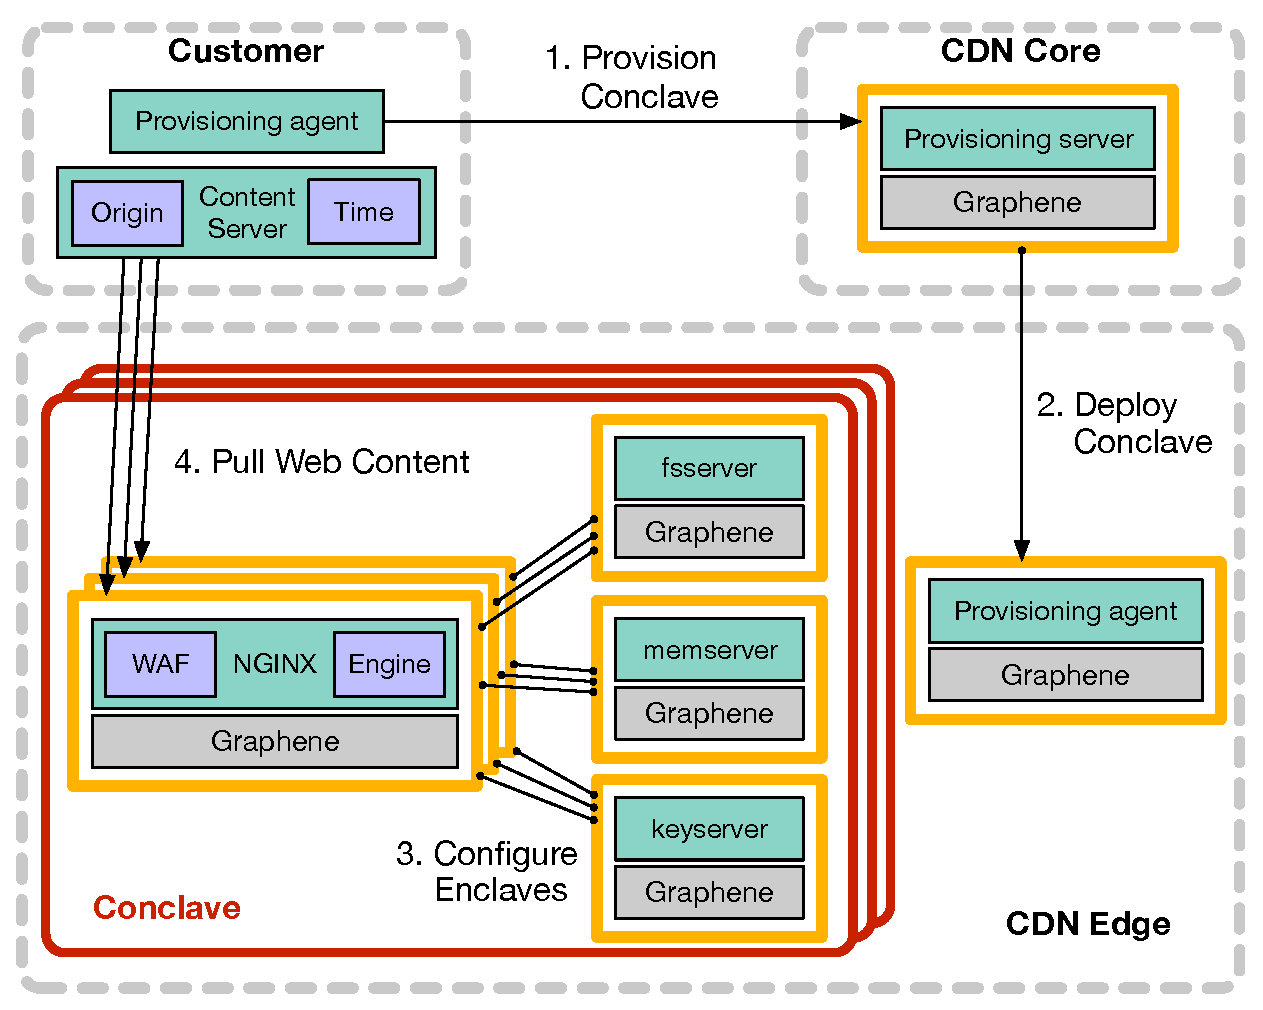
\includegraphics[width=0.48\textwidth]{figs/phoenix-design}
	\caption{Architectural design of \name. Multiple enclaves (yellow
	boxes) reside in a logical conclave (red boxes), permitting
	multiple processes and multi-tenant deployments. The CDN Edge and
	Core servers run on untrusted hosts.}
\label{fig:design}
\end{figure}

% }}}

The conclave design extends the open-source Graphene SGX libOS~\cite{graphene}
to support shared state abstractions among multiple processes.
%
Graphene~\cite{graphene} supports the critical system calls
\texttt{fork} and \texttt{exec} by automatically spawning a brand new
enclave, and performing a checkpoint-and-migration (essentially copying
the first enclave's memory pages into the second).
%
Graphene further offers some support for these separate processes
(enclaves) to communicate with one another over pipes, and implements
copy-on-write fork, signals, semaphores, message queues, and exit
notifications as RPCs over these pipes.
%
In other words, Graphene essentially turns a traditional multi-process
application into a ``distributed system'' of enclaves, along with some
basic plumbing to allow them to communicate with one another.


%% Key design challenges for libOSes include support for \texttt{fork} and
%% \texttt{exec}, and the subsequent management of shared state among the
%% processes.
%% %
%% Of the SGX-based libOSes, only Graphene supports forking, which it models as a
%% checkpoint and restore process migration.
%% %
%% In Graphene, multiple libOS instances coordinate over pipes to implement a
%% consistent, distributed POSIX abstraction, yet appear to the application as a
%% single, shared OS\@.  
%% %
%% In particular, Graphene implements copy-on-write fork, signals, semaphores,
%% message queues, and exit notifications as remote procedure calls (RPCs) over
%% these pipes.

However, two important multi-process abstractions that Graphene does not support with
confidentiality and integrity guarantees are a read-write filesystem, and
shared memory.
%
Graphene's sole filesystem, \texttt{chrootfs}, is modeled as a restricted view
of the host's filesystem.
%
%The contents of the filesystem are in plaintext; for read-only files, Graphene
%ensures the integrity of the file's contents by loading cryptographic hashes
%of the content into the enclaved libOS and verifying these hashes upon file
%reads; writable files have no integrity protections.
%
Graphene does not support shared memory at all (neither anonymous nor
file-backed).


Conclaves extend upon this prior design by leaning into the distributed
system nature of it.
%
We implement kernel services as \emph{kernel servers}; applications
act as clients, connecting to and issuing requests to kernel
services---via pipes or TLS network connections.
%
The kernel servers also run atop the libOS.
%
Our design is effectively that of a multi-server microkernel system,
similar to GNU Hurd or Mach-US, in which shared resource abstractions
are implemented as a set of enclaved daemons shared by all processes in
the system.
%% The daemons themselves also run atop the libOS\@.


\subsubsection{Conclave Kernel Servers}

Using the NGINX web server as a guide (as software representative of a
CDN edge server), we identified five key shared resources: files,
shared memory, locks/semaphores, cryptographic keys, and time.  
%
For flexibility in deployment configurations, we implement four servers
to manage these resources\footnote{Due to the common pattern of using
locks with shared memory, the memserver manages both.}:
%
We implement the fsserver, memserver, and keyserver as single-threaded,
single-process, event-driven servers that communicate with the application's
Graphene instances over a TLS-encrypted stream channel. 
%
The timeserver uses a datagram channel.
%
Each server is independent.


\parhead{fsserver}
%
For our file server, \emph{nextfs}, we extend lwext4's~\cite{lwext4} userspace
implementation of an ext2 filesystem into a networked server.
%
nextfs uses an untrusted host file as the backing store, similar to a block
device.
%
We develop three variants of this device to accommodate different security
postures, and a fourth for comparison purposes.

\vspace*{-0.5\baselineskip}
\begin{widelist}

\item 
%
\textbf{bd-std} stores data blocks in plaintext, without integrity
guarantees. This serves as a baseline in our evaluation.


\item
%
\textbf{bd-crypt} encrypts each block using AES-256 in XTS mode, the de
	facto standard for full-disk encryption~\cite{xts-ieee,xts-nist}.
%
We base each block's initialization vector on the block's ID.
%
This, too, lacks integrity guarantees, and is thus suitable only for an
	honest-but-curious attacker.


\item
%
\textbf{bd-vericrypt} adds integrity guarantees to bd-crypt, thus
	providing authenticated encryption.  It does so by maintaining a
	Merkle tree over the blocks: a leaf of the tree is an HMAC of the
	associated (encrypted) block, and an internal node the HMAC of its
	two children.
%
To keep the memory needs of the enclave small, bd-verity consults a
	serialized representation of the tree in a separate file, rather
	than use an in-memory representation.
%
The root of the Merkle tree exists both on the file and in enclave
	memory; the HMAC key exists only in enclave memory.
%
As an optimization for reducing reads and writes to the Merkle tree
	file, bd-verity maintains an in-enclave LRU-cache of the tree
	nodes.
	%
	bd-vericrypt is the appropriate choice in a Byzantine threat model.
	

\end{widelist}


\parhead{memserver}
%
We implement shared memory as filesystems that implement a
reduced set of the filesystem API\footnote{Graphene does not have a
unified filesystem and memory subsystem, and
thus \texttt{munmap} is not currently available as a filesystem operation.
}:
\texttt{open}, \texttt{close}, \texttt{mmap}, and \texttt{advlock}
(\texttt{advlock} handles both advisory locking and unlocking).
%
In our shared memory filesystems, files are called \emph{memory files}, and
either represent a pure, content-less lock, or a lock with an associated
shared memory segment.
% 
Memory files are non-persistent: they are created on the first open and
destroyed when no process holds a descriptor to the file and no process has the
associated memory segment mapped.


We implement three versions of shared memory.
%
Each stores a canonical replica of the shared memory at a known
location (either a particular server or file).
%% Each uses a scheme whereby a canonical replica of the shared memory is
%% stored at a known location.  
%
Upon locking a file, the client ``downloads" the canonical replica and updates
its internal memory maps.
%
On unlock, the client copies its replica to the canonical.
%
%Note that SGX does not provides a means for us to interpose on page accesses
%(as a page table handler would in normal Linux), and thus we must 
%interpose through the locking and unlocking system calls.
%\begin{widelist}

\vspace*{-0.5\baselineskip}
\begin{widelist}

\item 
%
\textbf{sm-vericrypt-basic} uses an enclaved server to keep the canonical
memory files in an in-enclave red-black tree.

\item 
% 
\textbf{sm-vericrypt} implements a memory file as two untrusted host files: a
mandatory lock file, and an optional segment file.
%
When a client opens a memory file, the sm-vericrypt server creates the lock file on the
untrusted host, and the Graphene client maps (\texttt{MAP\_FILE|MAP\_SHARED})
the lock file into untrusted memory.
%
The client then constructs a ticketlock structure over this untrusted shared
memory.
%
Since the untrusted host may manipulate the ticketlock's turn value, a
shadowed, trusted turn number is maintained by the enclaved sm-vericrypt
server.
%
After the client has acquired the lock, the client makes an RPC to the
server to verify the turn number.
%
The server thus acts as a trusted monitor of the untrusted monotonic
	counter.
%% As such, the server acts as a trusted, monotonic counter that monitors an
%% untrusted monotonic counter.


If a client \texttt{mmap}s the memory file, the server creates the
associated segment file on the untrusted host.
%
When the client subsequently locks the file, the client makes a \texttt{lock}
RPC to server, which returns the keying and MAC tag information for
the segment.
%
The client copies the untrusted memory segment into the enclave, and uses
AES-256-GCM to decrypt and authenticate the data.
% 
When a client unlocks the file, the client generates a new IV, copies an
encrypted version of its in-enclave memory segment into the untrusted
segment file, and makes an \texttt{unlock} RPC to the server, passing along
the new IV and MAC tag.

% \clg{I think this section can be compressed}

\item 
%    
\textbf{sm-crypt} 
	%is like sm-vericrypt, but 
	assumes the untrusted host does not
tamper with data.  As such, sm-crypt uses AES-256-CTR instead of AES-256-GCM,
and does not need an enclaved server to monitor the integrity of the ticketlock
and IV.

\end{widelist}




\parhead{keyserver}
%
The keyserver is an SGX enclave rendition of a hardware-security module
(HSM): the keyserver stores private keys and performs any private key
cryptographic operations.
%
Like Keyless SSL~\cite{keyless-ssl}, this not only maintains the
confidentiality of the private key with respect to an untrusted host,
but also isolates the key to an address space distinct from the
application's, thereby guarding against critical memory disclosure
vulnerabilities, such as Heartbleed~\cite{heartbleed-cve}.


We implement the keyserver as two components: the keyserver proper, and an
OpenSSL engine (``engine'' in Figure~\ref{fig:design}) that the application
loads as a shared library; the engine proxies private key operations to the
keyserver.
%
Unlike the fsserver and memserver clients, the key client operates at
the application layer, outside of Graphene.


OpenSSL's engine API requires the caller (in our case, NGINX) to provide an
\texttt{RSA} object, which contains the secret key.
%
To avoid having to expose the key, we modified OpenSSL to populate
\texttt{RSA} objects with dummy keys that instead serve as identifiers
that the keyserver uses to look up the real keys it stores securely.


To reduce the number of connections and avoid a dependency on the memserver for
lock files, our engine maintains the property that all keys for the same
keyserver, within the same process, share a single connection.
%
This requires that the engine detect forking by the application, which we
achieve by also associating process IDs with the \texttt{RSA} objects.


\parhead{timeserver}
%
Given that the components of a conclave must authenticate one another,
we need trusted time to guard against attacks that 
% manipulate the conclave's sense of time to
trick the conclave into accepting expired certificates.
%% (and therefore possibly
%% cracked) certificates.
%
Unfortunately, SGX itself does not provide trusted time.  
%
Its SDK~\cite{sgx-linux-sdk} provides features~\cite{sgx-trusted-time}
for retrieving coarse-grained, monotonic time through a protected clock
provided by Intel's Converged Security and Management Engine (CSME),
but not all processors support it~\cite{ayeks-sgx-hardware}.
%

%% Techniques that base wall-clock time on the \texttt{RDTSC} family of x86
%% instructions cause a \texttt{\#UD} fault in SGXv1, while in SGXv2 the
%% instruction may be modified by a hypervisor.
%% %
%% Intel's SGX SDK~\cite{sgx-linux-sdk} does provide
%% features~\cite{sgx-trusted-time} for retrieval of coarse grained, monotonic
%% time, through a protected clock provided by Intel's Converged Security and
%% Management Engine (CSME)\@.  
%% %
%% However, this feature relies on the presence of the CSME (not all processors
%% include this firmware~\cite{ayeks-sgx-hardware}), and moreover relies on an
%% enclave to securely obtain a base wall-clock time from a remote, trusted,
%% server.


Instead of relying on the CSME, we simply design a remote, signed
timestamping server.
%
The timestamping server runs outside of an enclave, on a remote trusted
machine (e.g., at the CDN's customer).
%
The timeserver's purpose is not to provide fine grained precision to
the conclaved processes, but rather to serve as an integrity check of
the time those processes receive from the untrusted host.

We modify the Graphene system call handlers for \texttt{getttimeofday},
\texttt{time}, and \texttt{clock\_gettime} to optionally proxy application
calls to a remote, trusted, timestamp signing server.
%
The use of such a timeserver, and the related parameters, such as the
timeserver's public key, are specified by the Graphene user (here, the content
provider), and hard-coded into Graphene's configuration.
%
As a freshness guarantee, each request includes a new, random
nonce, generated by the Graphene system call handlers.
%
The timeserver, in turn, returns an RSA signature over a message
consisting of the current time concatenated with this nonce.


%% As time-related system calls occur frequently in event-driven applications like
%% web servers, and as each timeserver request incurs latency due to both the
%% network and RSA operations, the Graphene client makes remote requests for  $p$
%% percent of the time-related system calls, where $p$ is a configurable
%% parameter.
%% %
%% Upon verifying a timeserver response, the Graphene client retrieves the time
%% as reported by the untrusted host, and verifies that the time the host
%% returns is within a configurable tolerance to the timeserver's time.
%% %
%% For a time-related call in which the Graphene client does not consult the
%% timeserver, Graphene checks that the time returned by the untrusted host is
%% greater than the last time value retrieved.


Our timeserver approach resembles Google's roughtime protocol~\cite{roughtime};
future work would fully port the roughtime protocol to Graphene to reduce the
need for a trusted timeserver by instead tolerating some fraction of
misbehaving servers.
%
Note, however, that, in the SGX setting, both our approach and roughtime are best
efforts; an untrusted host that identifies the traffic between the Graphene
client and timeserver could, for instance, ``slow down" time by delaying the
responses.



\subsubsection{Conclave Images} % {{{

Conclaves bundle the SGX microkernel runtime and application suite into a
deployable and executable image, reminiscent of a traditional container image.
%
When the conclave is executed, the first enclave process that is
executed is an init process, which executes the kernel servers and the
specified application proper.
%
From that point, the application can fork, spin up new applications,
and so on.


\subsubsection{Bootstrapping Trust} % {{{

%% Before we address provisioning secrets to the running conclave, we describe

We first address how the conclave, viewed as a distributed system,
establishes the trust of each member node, whether kernel server or
application process.
%
This is a chicken-and-egg problem of establishing a secure channel
between two nodes without first provisioning these nodes with, say,
private keys and certificates for mutual authentication.
%
%% 
%% 
%% %
%% There are two cases we must address: (1)~trust between a parent-child
%% relation (for instance, between the init and the processes it spawns),
%% and (2)~trust between non parent-child process relationships (such as
%% between the application nodes and the kernel servers).
%% %
%% In both cases, the problem boils down to a chicken-and-egg dilemma of
%% establishing a secure channel between two nodes without first
%% provisioning those nodes with, for instance, private keys and
%% certificates for mutual authentication.
%% %
%% If we can establish such a channel, then provisioning becomes
%% straightforward: NGINX servers can simply (and safely) read sensitive
%% key material from keyservers, and read and write sensitive user data in
%% the fsserver and memserver.



The standard approach for establishing a secure channel in an SGX setting is to use SGX
as a root of trust and enclave attestation as a form of authenticated identity,
and to merge this form of attestation into the establishment of the shared
channel secret.
%
To that end, \name follows closely from the work of Knauth et
al.~\cite{DBLP:journals/corr/abs-1801-05863}, which 
integrates attestations with TLS by adding the SGX quote as an X.509
certificate extension.
%
This has the effect of making channel establishment and SGX attestation
occur together,
atomically, with respect to the channel protocol.
%
%% prevents
%% man-in-the-middle attacks by making channel establishment and SGX
%% attestation occur together, atomically, with respect to the channel
%% protocol.
%% %
%% The core problem they address is that, to prevent
%% man-in-the-middle attacks, secure channel establishment and SGX attestation
%% must occur together, atomically, with respect to the channel protocol.
%% %
%% In order to do this, they integrate attestation with TLS by adding the SGX
%% quote as an X.509 certificate extension.
%% %
Certificate validation can thus be extended to examine these new extensions.


Adding new certificate extensions, of course, is not the full story.
%
In this setup, the enclave generates an ephemeral key pair.
%
SGX quotes are, mandatorily, over the enclave image, the enclave signer,
non-measurable state, such as the enclave mode (e.g., debug vs production),
and, optionally, any additional data (user data) the enclave wants to
associate with itself.  
%
The trick for ensuring the atomicity of attestation and secure channel
establishment is for the enclave to specify as user data a hash of the ephemeral
public key.
%
Since the key pair is created within the enclave, and since only an enclave can
get a valid quote, such user data binds the key pair to the enclave.
%
The enclave then generates a self-signed certificate for this ephemeral public
key, which includes the aforementioned extensions for the quote and IAS
verification.


In our conclave setup, the attestation is a local attestation, and validation of
the quote is based on a list of valid attestation values in the manifest.
%
Specifically, the manifest specifies a graph of which processes can establish
secure channels with one another.


\subsection{Evaluation}

\section{Codomains Introduction}
\label{sec:codomains-intro}

% the problem setup

When we build an application that requires the participation of mutually
distrustful parties, our choices are: 
%
\begin{enumerate}
    \item Run the entire application in a secure execution environment, such as
        a hardware enclave, or via translation to an MPC program.

    \item Distribute the application;  each party locally executes
        their sensitive piece of the computation.

    \item Hybrid, ``mix-mode", schemes whereby each party locally executes
        their sensitive piece of the computation, and jointly invoke a secure
        enclave or MPC scheme for computations that combine the parties'
        sensitive data.
\end{enumerate}


Our focus is designing and implementing operating system abstractions 
that enable developers to write such hybrid applications as if they were
monolithic, local applications.
%
This motivation is not conceptually different from that of 
remote procedure calls (RPCs):  with RPCs, developers code their applications
using the familiar procedure call, but the calling process and the
process containing the procedure being called execute on different
hosts.
%
To the application proper, the fact that the call involves cross-host I/O
is mostly transparent.
%
In our setting, the system abstractions define party-local and multi-party
secure computations, and the underlying system manages moving the execution
between the computation domains, maintaining resource consistency across
domains, and restricting information flow among domains.



As with RPCs, prior work in this area endeavors to hide the details of the
resultant distributed system from the application developer.  
%
Projects such as privtrans and Glamdring use developer-provided source code
annotations and static analysis to assist the compiler in partitioning the
monolithic application into separate programs.
%
In contrast, Fabric, Wysteria, and secure goroutines expose partitioning as
first-class language constructs, whereby developers programmatically indicate
which statements execute in a specific domain, and what data is accessible to
that domain.
%
In these systems, a trusted language runtime enforces isolation between
domains.


Similar to prior work, we want to maintain the source-level abstraction of
a monolithic program, but allow for dynamic, at run-time, mode switches.
%
Morever, we want to present a language-neutral mechanism for switching modes.
%
If mode-switching is dynamic and language-neutral, then orthogonal, application
interposition techniques, may be layered onto the system to increase the
transparency of the multi-domain environment with respect to the application.

\section{Codomains Background}
\label{sec:codomains-background}

We focus on two use cases that involve multiple parties cooperatively running
an application where the input of at least one party is confidential:
(1) outsourcing TLS-based applications to a third party, and (2) federated
analysis over private data.


\parhead{Outsourcing TLS applications}
%
In this setup, a company uses a third party, such as a cloud host or cloud
service, to operate an application server, such as for web, DNS, or mail.
%
Operationally, the status quo is for the company to shares or otherwise entrust
the third party with the application's private keys.
%
This has significant implications on the trust model of the PKI and the web
writ large, as these third parties can arbitrarily impersonate any of their
customer organizations.
%
Our goal is to design system primitives that allow developers to write or
patch, and deployers to configure, such applications with the property that the
company retains exclusive custody of its private keys.


\parhead{Collaborative Data Processing}
%
In this setup,  the aggregate dataset consists of the confidential, local,
datasets of multiple parties.
% 
The parties themselves might be mutually distrustful, or may simply be
prevented by law from sharing their data.
%
An analyst wants to process the datasets to determine some non-confidential
result.
%
With federated databases, the result may be the cardinality of an intersection
across the datasets.
%
With federated learning, the result may be the global model parameters (such
as the weights of a deep neural network), derived from the aggregation of the
parameters from each party's locally-trained model.
%
Our goal is to enable the developer to express, in a
single program, the multi-party nature of the application, with the underlying
system managing the application's distribution across parties. 


While our system will present an interface for partitioning the application
across the parties, partitionioning alone does not prevent private data
leakage.
%
For instance, local results and parameters may, by themselves, reveal
information about the private data samples.
%
Thus, orthogonal to our system, the application may additionally require
methods for achieving differential privacy, such as by adding a carefully
chosen amount of noise to the local results.


\subsection{Threat Model}

We assume an honest but curious (HbC) threat model: each party faithfully
executes the program, but may analyze their portion of the execution to try to
recover the private data of other principals.
%
We assume that the parties trust the application; that is, the application does
not deviate abitrarily from its stated purpose, and does not actively try to
leak sensitve data.
%
We assume that the application is bug-free, and thus our model omits external
actors, such as a remote attacker.


An HbC model is not inherent, but is reasonable for our use cases,
given the mutually beneficial incentives among the parties, and further
simplifies the system design.
%
Consider, in contrast, a more adversarial model where the parties, or the
application itself, may abuse the interface for domain switching---as by
switching at an unexpected state, or switching to a malicious code page---for
the purpose of actively leaking sensitive data. 
%
In this model, the target domains must first, externally, validate the
execution state against an expected starting condition before commencing
execution.


An interesting design point related to the threat model is whether the
application is globally public, or whether some portions are private and thus
confidential to a party. 
%
For instance, in the scenario of a company outsourcing a web server to a CDN,
the CDN's web server may be proprietary, and the CDN operator in turn may be
unwilling to allow the server's execution to switch to a company's domain
for fear of leaking proprietary knowledge.
%
Naively, this scenario reduces to specifying that private code pages should be
pinned to the owning domain, and that execution may switch domains only at
non-private points in the application's execution.
%
The tricky aspect is that the data written by private code pages should,
likewise, be private, as sharing such data pages could reveal aspects of
the private code.
%
We consider this feature as future work, but briefly revisit the idea in
\S\ref{sec:codomains-challenges}.


Typical of other work in this area, we consider side-channels out of scope.


%Within the realm of secure, federated data processing, the need for differential
%privacy is virtually unavoidable, as local results and parameters may, by
%themselves, leak information about the underlying data samples.
%%
%Differential privacy (DP) is a property of randomized queries that take a
%database as input and return a statistical result, such as an aggregate.
%%
%The database is a collection of rows, with each row containing data
%from one individual.
%%
%Informally, queries are differentially private if arbitrary changes to a single
%individual’s row result in only statistically insignificant changes in the
%function’s output distribution. 
%%
%Thus, the presence or absence of any individual has a statistically negligible
%effect.
%%
%Practical solutions for achieving DP typically rely on adding a carefully
%chosen amount of noise to the result.
%%
%DP offers a provable bound on the amount of information that an adversary can
%learn about any individual, even with access to auxiliary information


% DP Definition
%
%Differential privacy (DP): by
%disallowing certain qeuries and carefully adding a chosen amount of noise to
%the result of others, it is possible to give a strong upper bound on how mcuh
%an adversary could learn about an invididual person's data.
%


% such as an aggregate statistical value, or to learn the parameters to
%a machine learning model trained across the datasets.


%%%% FEDERATED LEARNING
%
%Federated Learning (FL) trains an algorithm across
%multiple principals holding local, confidential, data samples, thereby allowing
%the principals to build a common machine learning model withouth
%sharing their data.
%%
%%
%As local parameters may, by themselves, leak information about the underlying
%datasamples, FL may further incorporate DP or secure aggregation.


%DStress is a system that can efficiently perform computations on graphs taht
%contain confidential data. Dstress assumes that the graph is physically
%distributed across many participants, and that each participaint only knows a
%small subgraph; it protects privacy by enforcing tight, provable limits on how
%much each participant can learn about the rest of the graph.
%
%The motivating usefaul is measuring systemic risk in financial networks. The
%requried information is extrmeemly sensisive because it directly reflects the
%business strategy of each bank.
%
%It is well known taht many interesting thnigs can be learned by collecting and
%analyzing large graphs. Tools assume that the user has a property Graphen G
%(that is, a graph that has some data asscoiated with its vertixes and/or edges)
%and wishes to compute com function F(G) over this graph and itsp roperites.
%
%However, there is another class of use cases where the graph G contians
%sensitvie information and is spread across multiple administratigve daomins. In
%this situation, each domain knows only a subset of the vertexes and edges, so
%it cannot compute F(G) on its own, but the domains may not be willing to share
%their data with each other because of privacy concerns.
%
%
%DStress support vertex programs; it addresses the first challenge with a
%special graph-computation runtime tha can execute vertex programs in a
%distributed fashion, using MPC and a varint of ElGamal encryption
%(homomorphic for transferring data between domains, and it addresses the
%second challenge by keeping intermediate results encrypted at all times, nad by
%offering differential privacy on the final result.
%
%Our approach is based on two key insights. Our first observation is that much
%of the enormous cost of the MPC-based strawman comes from the fact that the
%graph is itself confidential and therefore must be an input to the computation.
%We can get around this by fomrulating the funciton F as a vertex program – that
%is, as a sequence of comptuations at each vertex that are interlevaed with
%message exchagnes over the edges – and by executing it in a distributed
%fashion. The main challenge is to prevent information leackage thorugh
%intermediate results. In DStress, we asccomplish this with a combination of
%secret sharing, small MPC invocations for the computations at each vertex, and a
%special protocol for transferring shares without revelaing the topology of the
%graph. our second key insight is that we can use differential privacy to
%achieve output privacy.



\section{Codomains Design}
\label{sec:codomains-design}

Our goal in this section is to explore the concept of cooperating execution
domains to arrive at an application programming interface (API)
for developing programs for such an execution model.
%
The core abstractions are pinning data to a domain and switching (migrating)
between domains, while the core challenges are providing resource
consistency and mechanism transparency.


\subsection{Coprocesses}

We first introduce the concept of a coprocess, its properties, and a
prospective API\@.
%
Abstractly, a coprocess is a process to which a client process yields its
execution.
%
By itself, this is not a novel idea: the \texttt{ptrace} system call allows one
process to control considerable aspects of another, while
\texttt{userfaultfd} allows one process to service another's page faults.
%
Orthogonally, runtime loading techniques, such as \texttt{LD\_PRELOAD}, enable
shims for proxing a process's library calls.


Our interest with coprocesses is handling, in userspace, services requisite to
codomains: distributed shared memory, distributed fileystems, and the
checkpointing and restoring of the client process, while further enabling both
explicit and implicit yields to these services.
%
In these respects, a coprocess is similar to a library operating system, but
one that operates in an address space distinct from its client process: instead of
trapping directly to the kernel, the process traps to its coprocess, which may
either service the trap on its own, or forward the trap to the kernel.


\parhead{Coprocess API}
%
In Listing~\ref{lst:coproc-api}, we present the coprocess API\@.
%
The API design presents the coprocess as an ambient service to the process
(similar to the kernel), abstracting away any details, or even notion, of IPC
between the coprocess and process.
%
A process becomes a coprocess by calling \texttt{coproc\_create}, whose
argument is a unique pathname identifying the coprocess, and whose return value
is a socket-like descriptor for communicating with future client processes.
%
A client process attaches to a coprocess by calling \texttt{coproc\_set}, passing as an
argument the path representing the coprocess.
%
A process may have at most one coprocess, and a coprocess may service multiple
processes.
%
A processes's coprocess, and the state of being a coprocess, are attributes
within a process's control block.


Up until this point, a library based on UNIX domain sockets would perfectly emulate the
coprocess API\@.
%
The distinctive, non-emulatable, component of the API is \texttt{coproc\_yield},
which suspends the calling process's thread and yields the process's execution
state to the coprocess.

\begin{lstlisting}[
    frame=single, 
    caption={Coprocess API},
    captionpos=b,
    label={lst:coproc-api},
]
int coproc_create(const char *path)
int coproc_set(const char *path)
int coproc_call(int msgtype, void *args, void *result)
void coproc_yield(void *args)
\end{lstlisting}

In the sections that follow, we discuss how codomains are implemented as
a library on top of the coprocess API.


\parhead{Coprocess Server}
%
Before delving into codomains, consider how switching execution between domains
would appear at the coprocess-level.
%
A process in domain A sets a coprocess and yields execution.
%
The coprocess checkpoints the process's thread and then makes a remote request
to a service in domain B\@.
%
B's service may either be a coprocess, or a service that executes a new
coprocess.
%
Regardless the service must also execute a stub program that first attaches to the
coprocess and then launches a loader that restores A's thread.
%
Any page faults during the restoration process trap to the coprocess on B,
which may request the page from the coprocess on A.


\subsection{Codomains}

In Listing~\ref{lst:isolating-key}, we start with a single-threaded, two-party
example in of isolating private key operations to a single domain,
\texttt{domain\_priv}; all other parts of the applications execute in the
initial domain, \texttt{domain\_pub}.

\begin{lstlisting}[
    frame=single, 
    caption={Isolating a private key to a domain},
    captionpos=b,
    label={lst:isolating-key},
    numbers=left,
    numberstyle=\tiny,
    xleftmargin=2em,
    framexleftmargin=1.5em,
    ]
int domain_priv;
int domain_pub;
char *key;

load_key(path) {
    domain_pub = co_switch(domain_priv)
    key = read_file(path)
    co_mempin(key)
    log(log_fd, "loading key (%s)", path)
    co_switch(domain_pub)
    return key;
}
 
sign(key, buf, buflen) {
     domain_pub = co_switch(domain_priv)
     signature = do_sign(key,buf)
     log(log_fd, "signed something");
     co_switch(domain_pub)
     return signature; 
 }

main(int argc, char *argv[]) {
    coproc_set("/srv/foo.coproc");
    domain_priv = co_attach(url, rspec)
    load_key(argv[1])
    sign(key, argv[2], strlen(argv[2]))
}
\end{lstlisting}


The process starts in \texttt{domain\_pub}.
%
The process sets its coprocess on line 23, and then attaches to 
\texttt{domain\_priv} on line 24.
%
The \texttt{url} argument to \texttt{co\_attach} specifies the coprocess server
for \texttt{domain\_priv}, and \texttt{rspec} describes the resources (such as
filesystem, open descriptors, memory pages) that \texttt{domain\_pub} exports
to \texttt{domain\_priv}.
%
Internally, \texttt{co\_attach} invokes \texttt{coproc\_call} to initiate the
connection.
%
The return value of \texttt{co\_attach} is a descriptor for the attached
domain; the descriptor only has meaning to the coprocess, and is not present
in the process's kernel-level file descriptor table.


On line 25, the process calls \texttt{load\_key}, which then invokes
\texttt{co\_switch} to switch to \texttt{domain\_priv}.
%
Internally, \texttt{co\_switch} invokes \texttt{coproc\_yield} to checkpoint
the thread on \texttt{domain\_pub} and restore the thread on
\texttt{domain\_priv}.
%
\texttt{co\_switch} returns a descriptor representing the domain that
initiated the switch.


Within \texttt{load\_key}, \texttt{domain\_priv} pins the memory pages storing
the private key by invoking \texttt{co\_mempin};
such pages are cloaked when executing in another
domain, and uncloaked when a thread executes in the caller's domain.
%
Internally, \texttt{co\_mempin} invokes\texttt{coproc\_call}, as the
coprocess is responsible for how the memory itself is labeled.
%
In Listing~\ref{lst:isolating-key}, the \texttt{load\_key} and \texttt{sign}
functions perfectly encapsulate the key's use, and thus  \texttt{co\_switch}
simply ``wraps" their invocation.


When a domain accesses a cloaked page, the result is a fault to the process's
coprocess.
%
The coprocess either treats the fault as a segmentation fault (likely
terminating the process), or as a page fault.
%
In the latter case, the coprocess handles the page fault by moving execution to
the domain of the page owner, as if the application implicitly called
\texttt{co\_switch}.
%
The application dictates fault semantics via \texttt{rspec}
when attaching to the codomain.


% XXX: compare to 9p protocol: http://man.cat-v.org/plan_9/5/intro
\begin{lstlisting}[
    frame=single,
    caption={Codomain API},
    captionpos=b,
    label={lst:codomain-api},
]
int co_attach(char *url, struct co_rspec rspec)
int co_switch(int fd)
int co_getrspec(int fd, co_rspec *rspec)
int co_setrspec(int fd, co_rspec *rspec)
\end{lstlisting}



\parhead{Resource sharing and consistency}
%
In the \texttt{load\_key} function of Listing~\ref{lst:isolating-key}, the
application calls \texttt{read\_file} on line 7,
which opens a file, reads in the contents, and then closes the file.
%
Suppose \texttt{domain\_pub} first tested if \texttt{path} existed;
would that test succeed?  
%
Beyond this simple example, suppose that \texttt{domain\_priv} created a
file; would \texttt{domain\_pub} be able to view it? 
%

% XXX: you need the prpocess on B to call co_setrspec() before execve() to
% specify the resources.

%
In Listing~\ref{lst:isolating-key}, the domains do not need to share the filesystem:
\texttt{domain\_pub} and \texttt{domain\_priv} have completely separate
filesystems, and path names may even clash between the two.



Similar issues exist for file descriptors.
%
For instance, in the example, \texttt{log} writes the log statements to a log
descriptor.
%
This descriptor could represent a terminal, a file, or a socket.
%
We may want the write to proxy the call back to \texttt{domain\_pub} (which
would be necessary in the socket case), or to perform the write locally, as by
``migrating" the underlying resouce from \texttt{domain\_pub} to
\texttt{domain\_priv} (which may be more appropraite for the terminal case).
%
In other words, \texttt{rspec} not only needs to say which resources
are shared, but also how they are shared.


In Listing~\ref{lst:codomain-api}, we present the complete codomain API\@.


\parhead{Distributed Shared Memory}
%\parhead{Multi-Threaded}
%
What happens in a multi-thread (or multi-process/shared memory), two-party
example.  
%
The core issue is that a thread on \texttt{domain\_priv} might be making changes to
the address space (cloaked or non-cloaked), and these changes must be
consistent with the threads on \texttt{domain\_pub}.
%
For instance, even in the key loading example, \texttt{domain\_priv} is
potentially allocating memory and then cloaking memory for the private
key---threads on \texttt{domain\_pub} must be aware of such address space
changes.
%
Similarly, threads on both domains may be interacting over shared memory.
%
This necessitates some form of distributed shared memory.



\parhead{Federated (Parallel)}
%
% TODO: give a code listing of a simple federated algorithm, such as private
% set intersection, or the millionaires problem.
%
For federated use cases, it is useful to have some notion of parallel
execution
%
In such cases, there's no need for DSM; each migrated thread can have it's own
private address space and own file system.
%
In this case, each thread passes back the results to the \texttt{domain\_pub}
as a return value, of sorts, rather than in shared memory.


In some cases, we want the reutrn vlaue to be blinded, as \texttt{domain\_pub}
will take the return values of from all the private domains and feed them into
an enclave for some private operation (such as private set intersection).  
%
A simple, perhaps naive approach, would be that the private domains encrpyt the
output using the public key of the enclave's domain.
%
This then brings up the question of how domains know of the existence of other
domains; in particular, must ``capabilities" for other domains be passed in the
\texttt{rspec}.


\begin{lstlisting}[
    frame=single,
    label={lst:lwc-parallel},
    numbers=left,
    numberstyle=\tiny,
    xleftmargin=2em,
    framexleftmargin=1.5em,
]
int snapfd;

thr_func(worker_fd) {
    main_fd = co_switch(domain_fd)
    val = lwcswitch(snapfd)
    co_switch(main_fd);
    return val
}

main() {
    enclave_fd = co_attach()

    snapfd = lwccreate()
    if (snapfd != -1) {
        open("data.dat");
        val = do_work()
        encrypt_to_enclave(val)
        lwcswitchdicard(val);
    } 

    for 1 to N:
        pthread_create(thr_func, worker_fd)
            
    vals  = join_all_threads()
     
    main_fd = co_switch(enclave_fd)
    sum = secure_sum(vals)
    co_switch(main_fd)
}
\end{lstlisting}


\subsection{Enclaves as Codomains}
\label{sec:enclaves-as-codomains}
% TODO: it will be non-obvious to the audience how this would even work,
% so briefly sketch the design.



\subsection{Data-Directed Switching}
\label{sec:data-directed-switching}

There are two cases where, rather than explicitly calling
\texttt{co\_switch}, a party needs a process to implicilty invoke
\texttt{co\_switch}: (1) the private data cannot be encapsulated in a
functional interface, and (2) the application is a black-box; the
party's only knowledge of the application is that it requires a private input,
say a file.


The idea is that files are marked as pinned in \texttt{rspec}; access to the file faults the
thread to the owner domain, which then uses taint-tracking to determine the
propagation of the file's sensitive data throughput memory.
%
As memory is tainted, the taint-tracker invokes \texttt{co\_mempin} to 


pages that should be tainted.
%
The thread then migrates back when attempting to access some data pinned by
another domain, or after so many instructions have occurred sequentially over
non-pinned data.


The issue that comes up is that, in order to make progress, there needs to be
declassification of pinned data; for instanace, a signature would be marked as
pinned by taint-tracking, but must be declassified.
%
This requires, in some form, hooking the returns from such functions.
%
In a way, this a form or \emph{half-wrap} in that the domain conceivably could
be migrated to at any point, but has well defined exit points and exit
conditions.



\subsection{Potentional Issues}

We need to be aware of deadlock arising from join computations over resoures
pinned by distinct domains.
%
This is likely a programming error, as such computations should occur in a
secure enclave.



% TODO: for MEM_PIN_SWITCH, what is the resource_spec?

% TODO: how is the pinned domain marked in the page table?  (a unique
% memory protection key):.

% TODO: what does the target argumet to switch() look like?  In other words,
% how are domains represented form the application's point of view?
%
%
% TODO: what would happen if the filesystem needed to be shared?
%
% TODO: what happens if pinned data is written to a descriptor/file?



% TODO: try to translate switch() into a "remote" lwc:
%  
%   fd = lwccreate(resource_spec)
%   ret = lwcswitch(fd)
%   if (parent):
%       switch
%       migrate
%   else:
%       

%   Antoher issue is that reads and writes to the file must subsequently be
%   kept in sync with any toher processes using that file on src. 
%    
% - What happens if dst tries to read/write a descriptor that was opened on src?
%
%   Similar situation where the file either needs to migrate to dst or the
%   calls proxied.
%
%   You can think of migrate() of being like a fork, and specifing which file
%   descriptors are kept open and which are closed across the join.  Or similar
%   to the mem_pin, src would pin the desripotrs, saying that access should
%   either fault, migrate back, or be proxied.
%
%   For the crypto and federated examples, there's no need for sharing
%   filedescriptors and files.
% 
%   - suppose domian_priv forgot to close the file descriptor as part of
%     read_file -- would that descriptor then be open in domain_priv?

\section{Codomains Evaluation}
\label{sec:codomains-eval}

\subsection{Correctness}
%
I need to ensure that a process running on Gemini shows the correct behavior
(program correctness), the isolation of pinned data (security correctness), and
the accuracy of the firewall rules (again, security correctness).
%
Pragmatically, this amounts to writing unit tests.
%
Additionally, it may involve showing generality by, for instance, instrumenting
more than just OpenSSL (the macro-benchmarks can also help to show generality
at the application-level).
%
For demonstrating data isolation, you might have an external program that just
dumps and scans a process's memory for a given byte string.


% TODO: try to think of a few correctness conditions, and what the unit test
% would look like for each one.  You might also consider tests for different
% application models, such as a single-threaded vs multi-threaded, vs
% multi-process application.


\parhead{Fault-injection tests}
%
TODO: purposefully try to send packets that do not pass the tag-aware packet
filters and verify that the filters prevent the transmission.


\subsection{Performance}

\subsubsection{Micro-benchmarks}

\parhead{What is the overhead of migration?}
% The idea is:
%   - understand the mechanics of migration and "profile" each of its steps.
%       - this might point out certain optimizations
%   - compare to alterntavies
%       - to understand tradeoffs/overheads compared to alternatives
%
Suppose a thread migrates to a target machine that has pinned a private key in
order to compute a signature with that key.
%
At the network level, how would a packet capture of the migration compare to
that of an alternative RPC-based implementation, such as keyless SSL\@?
%
In particular, how much traffic and how many round-trips does migration incur,
what is the purpose of each round-trip, and what is the corresponding ratio of
goodput to throughput?
%
Moreover, is each migration identical?


Closely related to the previous question, we seek to measure the latency of
migration and the related operations.
%
Direct overhead costs include network latency, while indirect costs include the
operations of checkpointing and restoring threads, as well as any TCP queuing
delays incurred by the source machine while its threads are paused, waiting for
the migration to return.


\subsection{Experiments}

We measure the performance of several $n$-party example programs of our own
design and drawn from the literature.
%
The \emph{richest} protocol copmutes the richest principal.
%
The \emph{GPS} protocol computes, for each participating principal, the other
principal that is nearest ot their location; everyon learns their nearest
neighbor without knowning anyone's exact location.
%
The \emph{Auction} protocol computes the high bidder among a set of
participating principals, as well as teh second-hgihest bid, which is revealed
to everyone; only the auction holder learns who is the winning bidder.
%



\subsubsection{Macro-benchmarks}

% nginx: apachebench
% bind, knot DNS, nds: dnsperf
% exim, postfix, qmail, sendmail: smtp-source
%
Give our use-cases of an HTTPS, DNS, and mail server, we stress test an
implementation of each server running in a standard Linux environment, and
compare request throughput and latency to the server running on top of Gemini.
%
Specifically we stress test the NGINX webserver using ApacheBench, the BIND DNS
server using \texttt{dnsperf}, and the postfix mail server using
\texttt{smtp-source}.


For each server, we benchmark several deployment scenarios.
%
In particular, does the deployment have only the organization pinning data (one
or more private keys), or does the service provider itself also pin data (such
as a spam or web application firewall rules).
%
In the former case, only the organization runs a process-monitor.


Furthermore, does the service support only one organization, or multiple?
%
For instance, the NGINX webserver can virtually host many sites, and thus,
under Gemini, could migrate to different organizations based on the request.
%
The application server might also support different server models, such as
multi-process or multi-threaded.
%
In a multi-process, multi-tenant configuration of NGINX, each worker process
is single-threaded and could migrate to a different organization
simultaneously, whereas in a multi-threaded configuration, only a single thread
could migrate away from the service provider any time.

\section{Conclusion}
\label{sec:conclusion}
% restate: 
%   - problem
%   - work you have done to solve this
%   - work you propose
%   - what success means

In this proposal, I discuss the problem of running applications that
assume a monolithic trust setting under conditions where that assumption no
longer holds, as due to a multi-party deployment or input data.
%
I posit that a major difficulty in solving this problem is the lack of support
that operating systems and programming languages offer for expressing
computation over an execution model that involves heterogeneous trust.
%
My approach is to apply operating system designs and fine-grained information
flow control techniques to hoist, or otherwise partition, the execution
environment into trust boundaries, thereby making the details of moving the
execution between trust domains, and restricting information flow among domains, a
concern of the run-time execution environment, rather than the application
developer.
% 
A primary goal of this approach is to keep the changes to the execution environment
transparent to the applications, such that these techniques allow for
\emph{post-hoc} refinements of a legacy application's trust model.
% 
I describe my prior work of enhancing library operating system for Intel SGX
enclaves,and propose codomains, an execution model that allows an application to
dynamically switch execution to different domains.
%
If successful, I will enable application deployment options that preserve
the privacy of the involved parties, as well as support the development of
applications that securely leverage the collective value of private data sets.


\bibliography{confs_long,main}
\bibliographystyle{acm}
\end{document}
